\graphicspath{ {../img/} }

\subsection{Шифрование сообщения}
Схема шифрования сообщения, разбиваемого на блоки:
\begin{center}
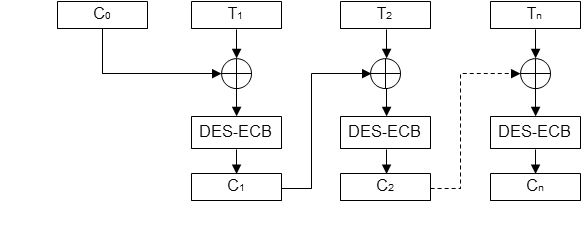
\includegraphics[scale=0.5]{des_CBC_cipher}
\end{center}
На данной схемме:
\begin{itemize}
\item $T_i$ \-- блоки исходного сообщения;
\item $С_i$ \-- блоки после шифрования;
\item $С_0$ \-- синхропосылка;
\item $DES-ECB$ \-- алгоритм шифрования блока;
\end{itemize}

\subsection{Шифрование блока}
Операция шифрования производится над блоком данных, размер которого равен 64 битам.
\begin{center}
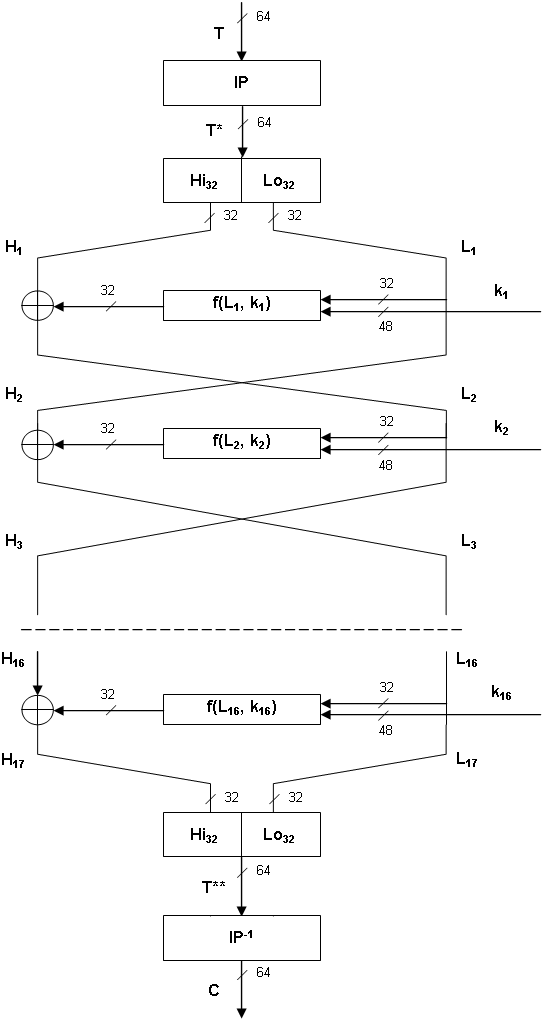
\includegraphics[scale=0.5]{des_ECB}
\end{center}
На данной схемме:
\begin{itemize}
\item $IP$ \-- перестановка бит, новый порядок определяется по таблице:
%% set columns = 8
%% set array = const.ip
%% include 'templates/table.tex'
\item $H_i$, $T_i$ \-- разбиение блока на 2 по 32 бита;
\item $\bigoplus$ \-- сложение по модулю 2 (xor);
\item $f$ \-- функция Фейстеля (см. ниже);
\item $k_i$ \-- ключевой элмент (см. ниже);
\item $IP^{-1}$ \-- перестановка бит в порядке:
%% set array = const['ip-1']
%% include 'templates/table.tex'
\end{itemize}


\subsection{Функция Фейстеля}
С ключевым элементом (48 бит) и половиной блока (32 бита) производятся действия:
\begin{center}
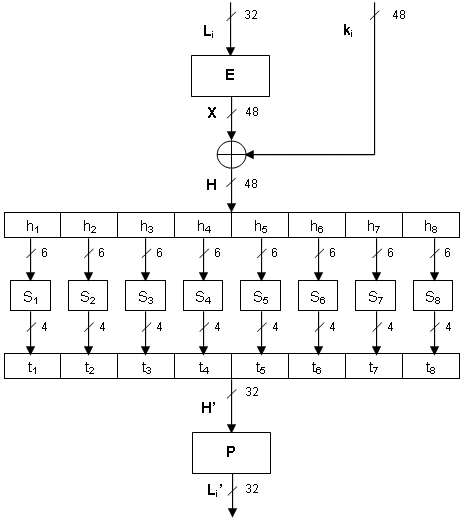
\includegraphics[scale=0.5]{des_f}
\end{center}
На данной схемме:
\begin{itemize}
\item $E$ \-- расширение (перестановка с повторениями) бит блока в порядке:
%% set array = const.e
%% include 'templates/table.tex'
\item $\bigoplus$ \-- сложение по модулю 2 (xor);
\item $h_i$ \-- 6-битовые блоки;
\item $P$ \-- перестановка по таблице:
%% set array = const.p
%% include 'templates/table.tex'
\item $S$ \-- операция замены 6-битового блока на 4-битовый по таблице (см. ниже),
где номер строки получают из 1-го и 6-го битов, а номер столбца \-- из битов 2..5: \\
%% set columns = 16
%% for array in const.s
    $S_\VAR{loop.index}$:
    %% include 'templates/table.tex'
%% endfor
\end{itemize}

\subsection{Получение ключевых значений}
В блок из 56 бит ключевой фразы добавляют биты чётности (по 1 на байт), а затем выполняются действия по схеме:\\
\begin{center}
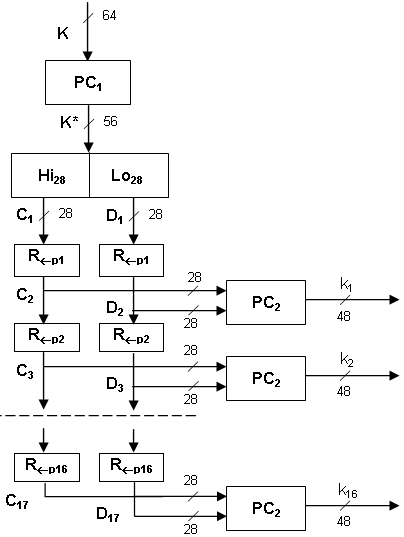
\includegraphics[scale=0.5]{des_key}
\end{center}
На данной схемме:
\begin{itemize}
\item $PC_1$ \-- перестановка битов ключа по таблице:
%% set columns = 8
%% set array = const.pc1
%% include 'templates/table.tex'
\item $C_i$, $D_i$ \-- разбиение ключа на 28-битные блоки;
\item $\leftarrow p_i$ \-- циклический сдвиг влево на $p_i$ бит, $p_i$ зависит от итерации и определяется по таблице:
%% set columns = 16
%% set array = const.shift
%% include 'templates/table.tex'
\item $PC_2$ \-- перестановка битов ключа по таблице:
%% set columns = 8
%% set array = const.pc2
%% include 'templates/table.tex'
\item $k_i$ \-- ключевой элемент для итерации i.
\end{itemize}